\section{Дубликатный маджонг}

\begin{additional}

В этом разделе описаны правила \textit{дубликатного} риичи-маджонга. В этой разновидности игры игроки на нескольких столах играют один и тот же расклад, чтобы потом выяснить, кто сыграл лучше.

\subsection{Начальная расстановка тайлов и порядок игры}

В дубликатном риичи-маджонге стартовые руки и стены выглядят следующим образом:

\begin{itemize}
	\item 4 стартовые руки по 13 тайлов,
	\item 4 стены по 18 тайлов каждая,
	\item мертвая стена из 12 тайлов.
\end{itemize}

\begin{figure}[H]
	\centering
	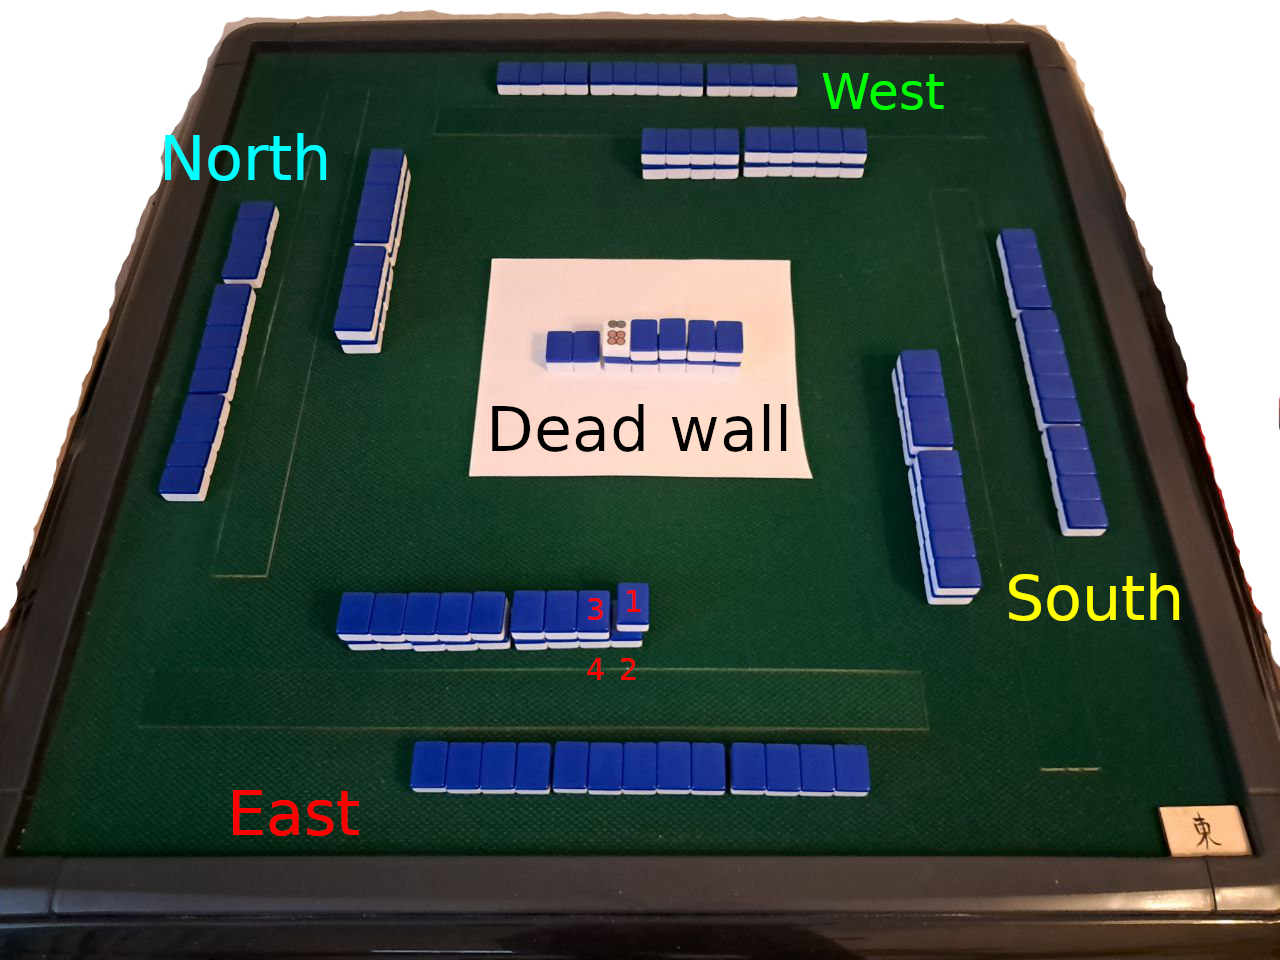
\includegraphics[width=8cm]{img/duplicate_start.png}
	\caption{Начальная расстановка тайлов для игры в дубликатный риичи-маджонг}
\end{figure}

\textit{В обычном риичи-маджонге при отсутствии объявлений игроки, сидящие на востоке и юге, возьмут по 18 тайлов, а игроки на западе и севере~--- по 17. Это число может меняться в случае объявления чи, понов и канов.}

В дубликатной версии у каждого игрока есть своя стена размером в 18 тайлов. Игроки всегда берут тайлы \textbf{из своей стены}, как после обычного взятия, так и в случае взятия тайла замены после кана. На картинке выше можно видеть пример стартовой расстановки, для игрока на востоке подписано, какой тайл он берет первым, вторым, третьим и четвертым.

\vspace{0.3cm}

Если \textbf{следующий} игрок не сможет взять тайл со своей стены (т.к. она пустая), то взятие и сброс текущего игрока считаются последними (и являются хайтеем/хотеем). На этом сбросе нельзя делать никаких объявлений, кроме объявления победы, а если объявления победы не последовало, то раздача заканчивается вничью.

\vspace{0.3cm}

Если в стене игрока не осталось тайлов, этот игрок не может объявить кан любого вида (потому что тайл замены брать неоткуда).

\vspace{0.3cm}

Если у следующего игрока в стене не осталось тайлов, текущий игрок может объявить чи, пон или (если у него остались тайлы в стене) кан. При выигрыше на тайле замены после кана, как и в обычном риичи-маджонге, хайтей не засчитывается, только риншан кайхо. Сброс этого игрока после объявления будет являться хотеем.

\vspace{0.3cm}

Если у текущего игрока стена закончилась, то он может сделать объявление пона с тоймена, если у камичи еще остались тайлы в стене, либо с шимочи, если у тоймена еще остались тайлы в стене. Объявление чи или пона с камичи невозможны, потому что сброс камичи по определению является последним (т.к. у текущего игрока стена закончилась).

\vspace{0.3cm}

Риичи можно объявлять только в том случае, если после сброса в стене каждого из игроков останется хотя бы по одному тайлу.

\vspace{0.3cm}

Мертвая стена имеет размер 12 тайлов. Из них два тайла вообще никак не участвуют в игре, а оставшиеся 10 являются индикаторами дор и урадор.

\subsection{Описание ханчана}

Каждый ханчан в дубликатной версии состоит из 12 раундов, обозначающихся от East 1 до West 4. Повторов дилера нет. На каждом столе в турнире эти раунды могут играться в произвольном порядке, но все 12 должны быть сыграны.

\vspace{0.3cm}

\textit{Мотивация выбрать 12 раундов происходит от того, что в среднем ханчан в риичи-маджонг длится чуть меньше 11 раундов, в зависимости от количества повторов дилера, а также от того, что игра должна быть сбалансирована, т.е. каждый игрок одинаковое число раз должен побывать каждым ветром в игре.}

\vspace{0.3cm}

Пример. Пусть в турнире участвуют 24 человека. Тогда последовательность сыгранных раздач в ханчане за разными столами может выглядеть так:

\begin{itemize}
	\item 1 стол: E1, E2, E3, E4, S1, S2, S3, S4, W1, W2, W3, W4.
	\item 2 стол: E3, E4, S1, S2, S3, S4, W1, W2, W3, W4, E1, E2.
	\item 3 стол: S1, S2, S3, S4, W1, W2, W3, W4, E1, E2, E3, E4.
	\item 4 стол: S3, S4, W1, W2, W3, W4, E1, E2, E3, E4, S1, S2.
	\item 5 стол: W1, W2, W3, W4, E1, E2, E3, E4, S1, S2, S3, S4.
	\item 6 стол: W3, W4, E1, E2, E3, E4, S1, S2, S3, S4, W1, W2.
\end{itemize}

\vspace{0.3cm}

Для каждого игрока выделяется его стартовый ветер. Это тот ветер, на котором он играет раздачи E1, S1, W1. Он определяет, какой ветер будет у игрока во всех остальных раздачах.

\vspace{0.3cm}

Следующая таблица указывает, на каком ветре в каком раунде сидит какой игрок в зависимости от его стартового ветра:

\begin{tabular}{|c|c|c|c|c|}
	\hline
	& \multicolumn{4}{c|}{Стартовый ветер} \\
	\hline
	Раунды & East & South & West & North \\
	\hline
	E1, S1, W1 & \textbf{E} & S & W & N \\
	\hline
	E2, S2, W2 & N & \textbf{E} & S & W \\
	\hline
	E3, S3, W3 & W & N & \textbf{E} & S \\
	\hline
	E4, S4, W4 & S & W & N & \textbf{E} \\
	\hline
\end{tabular}

\vspace{0.3cm}

Пример. Пусть стартовый ветер игрока~--- север, и он сидит на 6 столе в схеме последовательности раздач, указанной выше. Тогда в первой его раздаче (W3) он будет сидеть на юге, во второй раздаче (W4)~--- на востоке, в третьей раздаче (E1)~--- на севере, в четвертой (E2)~--- на западе, и т.д.

\subsection{Итоги раздач и подсчет очков}

По завершении каждой раздачи ее итог (кто сколько очков заработал или потерял) записывается в протокол. В случае, если на столе осталась риичи-палочка, каждый игрок плюсует себе 250 очков за каждую палочку. \textit{Смысл этого таков~--- палочка, оставшаяся на столе, в обычном риичи-маджонге переходит в следующую раздачу, здесь же каждая раздача должна начинаться в одинаковых условиях, поэтому каждая палочка на столе делится поровну между игроками.}

\vspace{0.3cm}

Подсчет очков для конкретного игрока за конкретную раздачу происходит следующим образом. Берутся результаты всех игроков, сидевших за этой раздачей на одном и том же стартовом ветре. Считается среднее этих результатов. Результат для игрока~--- это разница между его результатом и средним результатом.

\vspace{0.3cm}

Пример. Пусть в турнире участвует 24 человека, т.е. играется 6 столов. Пусть 6 игроков, стартовавших раздачу на одном и том же стартовом ветре, закончили ее с такими результатами: -2000, 0, 2000, 2000, 2600, 8000. Среднее этих результатов равно 2100. Таким образом, отклонения от среднего для этих 6 игроков равны -4100, -2100, -100, -100, 500, 5900.

\vspace{0.3cm}

Для каждой из 12 раздач такие отклонения от среднего суммируются и формируют итоговый результат игрока в ханчане. А результат в турнире~--- это сумма результатов во всех его ханчанах.

\vspace{0.3cm}

Возможно также конвертирование отклонений от среднего в другую шкалу, называемую IMP (International Match Points, по аналогии со спортивным бриджем):

\begin{tabular}{|c|c|}
	\hline
	Отклонение от среднего & IMP \\
	\hline
	0-400 & 0 \\
	\hline
	400-900 & 1 \\
	\hline
	900-1500 & 2 \\
	\hline
	1500-2200 & 3 \\
	\hline
	2200-3100 & 4 \\
	\hline
	3100-4200 & 5 \\
	\hline
	4200-5500 & 6 \\
	\hline
	5500-6900 & 7 \\
	\hline
	6900-8400 & 8 \\
	\hline
	8400-10100 & 9 \\
	\hline
	10100-12000 & 10 \\
	\hline
	12000-14000 & 11 \\
	\hline
	14000-16000 & 12 \\
	\hline
	16000-18000 & 13 \\
	\hline
	18000-20000 & 14 \\
	\hline
	20000-22000 & 15 \\
	\hline
	22000-24000 & 16 \\
	\hline
	24000-26000 & 17 \\
	\hline
	26000-28000 & 18 \\
	\hline
	28000-30000 & 19 \\
	\hline
	> 30000 & 20 \\
	\hline
\end{tabular}

\vspace{0.3cm}

В случае использования IMP в примере игроки вместо -4100, -2100, -100, -100, 500, 5900 очков получили бы -5, -3, 0, 0, 1, 7 IMP соответственно.

\vspace{0.3cm}

Также возможны командные турниры. Команда состоит из 4 человек, и матч между 4 командами проходит на 4 столах, где все игроки одной команды имеют различные стартовые ветра. После завершения всех ханчанов на этих 4 столах результаты игроков каждой команды суммируются и прибавляются к общему результату команд.

\vspace{0.3cm}

В случае использования IMP и равенства IMP по итогам турнира определение мест происходит по сумме отклонений от среднего. Если же и суммы отклонений от среднего совпадают, происходит дележ мест.

\subsection{Порядок проведения игр}

Перед каждым ханчаном организаторы турнира должны подготовить 12 раскладов и пронумеровать их от East 1 до West 4. На рубашку каждого тайла необходимо наклеить стикер, обозначающий, где этот тайл должен лежать в стене.

Один из примеров обозначения приведен на картинке:

\begin{figure}[H]
	\centering
	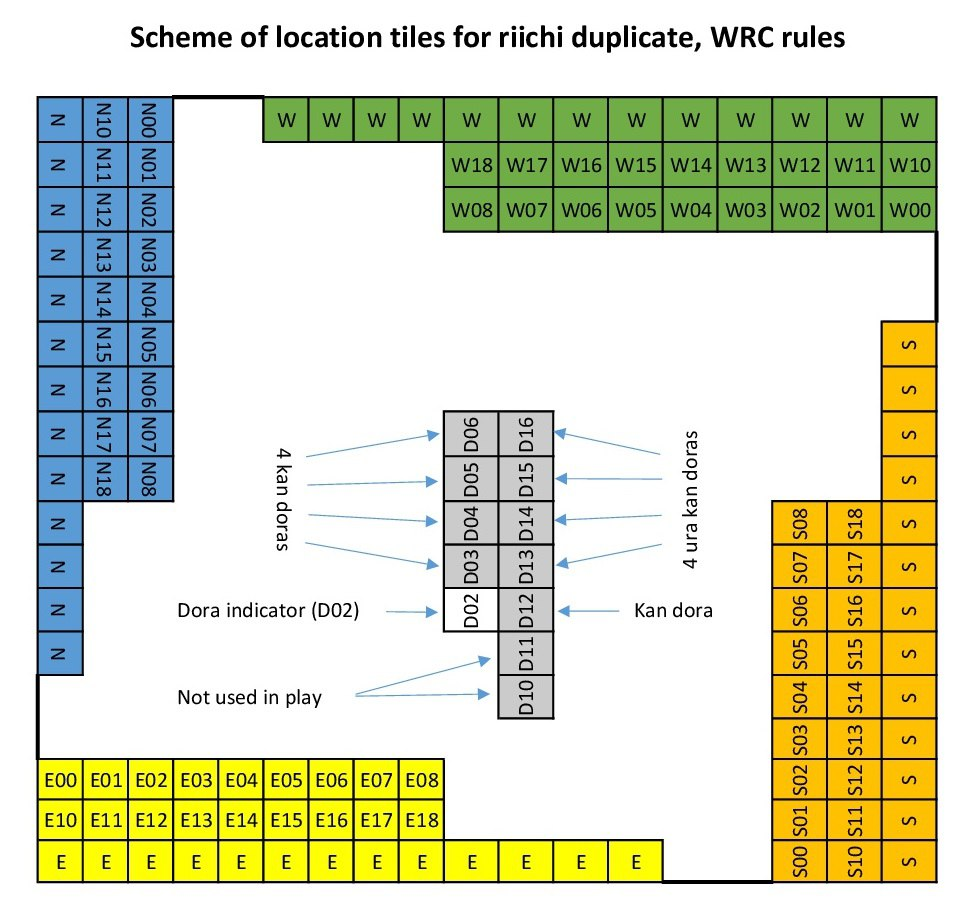
\includegraphics[width=8cm]{img/duplicate_marks.jpg}
	\caption{Пример обозначения тайлов для игры в дубликатный риичи-маджонг}
\end{figure}

Здесь стартовые тайлы игроков обозначены как ``E'', ``S'', ``W'' и ``N'', тайлы стен игроков пронумерованы от ``X00'' до ``X08'' (верхний ряд) и от ``X10'' до ``X18'' (нижний ряд), где ``X'' обозначает ветер (``E'', ``S'', ``W'' и ``N''), а тайлы мертвой стены от ``D02'' до ``D06'' (верхний ряд) и от ``D10'' до ``D16'' (нижний ряд).

\vspace{0.3cm}

Как вариант, вместо буквенных обозначений ветров и мертвой стены можно использовать маркеры разных цветов, например так:

\begin{itemize}
	\item тайлы востока~--- красный,
	\item тайлы юга~--- желтый,
	\item тайлы запада~--- зеленый,
	\item тайлы севера~--- синий,
	\item тайлы мертвой стены~--- черный.
\end{itemize}

Цвет маркеров не принципиален, главное, чтобы цвета были различимы между собой, и игроки знали и понимали, какой цвет что означает. Числовые обозначения также могут быть другими, главное, чтобы было понятно, где какой тайл должен находиться в стартовом раскладе.

В случае использования другой нумерации, если одновременно используются числа 6 и 9, около них необходимо ставить точку, чтобы их не перепутать.

\vspace{0.3cm}

Каждая раздача ставится на переносную доску. Организаторы приносят игрокам очередную раздачу, игроки ее играют, записывают результат и возвращают тайлы в стартовое положение согласно маркировкам на стикерах. После этого организаторы забирают доску с раздачей, и в будущем она отправится на другой стол, где ее разыграют другие игроки, а текущему столу приносят другую доску со следующей раздачей.

\vspace{0.3cm}

Можно использовать и другой вариант: расставить 12 столов, а участникам, сыгравшим свою раздачу, пересаживаться за следующий. В этом случае от организаторов не требуется забирать и приносить доски с раздачами за столы. Тем не менее, этот способ не рекомендуется, так как есть высокая вероятность, что игроки могут случайно или намеренно подсмотреть в чужие руки и получить информацию о раздаче.

\subsection{Нарушения и штрафы}

При получении чомбо провинившийся участник штрафуется на 20000 очков либо 15 IMP, в зависимости от того, какая схема начисления очков принята на турнире. При этом раздача аннулируется одним из двух следующих способов:

\begin{itemize}
	\item либо она аннулируется полностью за всеми столами,
	\item либо она аннулируется только на этом столе (все игроки, кроме провинившихся, получают 0 очков / 0 IMP), а среднее на остальных столах будет рассчитываться без учета этой раздачи (например, если столов в турнире 6, то знаменатель дроби при вычислении среднего будет не 6, а 5).
\end{itemize}

\vspace{0.3cm}

Если чомбо произошло одновременно на более чем половине столов с одинаковыми раздачами, следует в любом случае аннулировать эту раздачу за всеми столами (применить первый из двух способов аннулирования).

\vspace{0.3cm}

В случае неправильной рассадки все игроки, что сели неправильно, получают чомбо, а раздача аннулируется.

\vspace{0.3cm}

В случае неправильного расположения тайлов, если это невозможно исправить без последствий для проведения раздачи, игроки, в чьей стене тайлы были расположены неверным образом, получают чомбо, а раздача аннулируется. За корректность расположения тайлов в мертвой стене отвечает дилер. В любом случае, перед тем, как был сделан первый ход, всем игрокам следует проверить расположение и маркировку тайлов, чтобы исключить вероятность аннулирования раздачи и получения штрафа.

\vspace{0.3cm}

В случае взятия тайла не из своей стены, если это заметили сразу же (до встраивания тайла в руку), провинившийся участник получает фиксированный штраф (рекомендованный размер штрафа~--- 2000 очков / 3 IMP), иначе он получает чомбо, а раздача аннулируется.

\end{additional}
